\subsection{Explain different physical mechanisms, which can lead to molecular binding between atoms. Which type of molecular potentials can be expected? Discuss approximations to these potentials.}


Generelt er der to mekanismer, som gør at molekylære bindinger opstår mellem to neutrale atomer og lader dem sammen danne et stabilt molekyle. Vi vil se, at disse både afhænger af de specifikke atomer, men også af afstanden mellem de to kerner $R$, som set på \cref{fig:Q19_ReasonsForMolecularBinding}: Kemiske bindinger, som opstår idet, at atomernes orbitaler overlapper, og multipolvekselvirkningen, som opstår idet, at atomers opførsel som magnetiske dipoler vekselvirker med hinanden. Af kemiske bindinger vil vi kigge på de \emph{kovalente bindinger}, og af multipolvekselvirkningerne vil vi kigge på \emph{Van der Waals-bindinger}.\footnote{
    Ydermere findes der også følgende bindingstyper:
    \begin{itemize}
        \item \emph{Ionbindinger} (eng. ionic bond) opstår mellem positive og negative ioner, hvis der sker en udveksling af en (eller flere) elektroner fra atom A til  således, at atom A har en lavere elektrondensitet og B en større densitet.
        \item \emph{Hydrogenbindinger} (eng. hydrogen bond) opstår idet at der sker en ladningsforskydning mellem atomet X, som hydrogen er bundet til, og hydrogen selv, så f.eks. for vand ($\text{H}_2\text{O}$, hvor elektroner bindes tættere til oxygen end hydrogen, hvorfor der forekommer en polarisation af vandmolekylet. Hydrogen ser altså mere positiv ladning end negativ, da dens elektronsky er forskubbet mod oxygen. Et andet vandmolekyle vil derfor have lyst til at binde sig med en hydrogenbinding til det første vandmolekyle således, at det svagt negativt polariseret oxygen-atom fra det andet vandmolekyle binder sig med det svag positivt polariserede hydrogen-atom fra det første molekyle. For bindinger mellem hydrogen og et andet alkalimetal er polarisationen omvendt, så hydrogen bliver negativt polariseret, da alkalimetaller binder elektronerne svagt.
    \end{itemize}
}

\begin{figure}[!h]
    \centering
    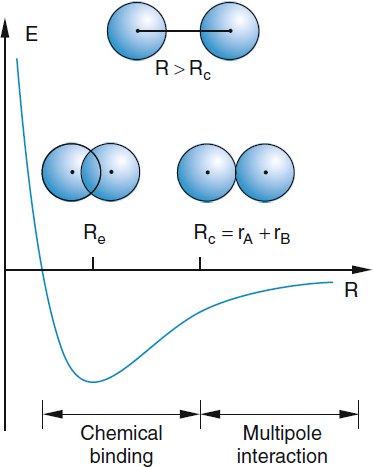
\includegraphics[width=0.45\textwidth]{Q19/images/ReasonsForBinding.PNG}
    \caption{Kemisk binding med overlab mellem atomorbitalerne er vigtig for $R < R_c$, hvor $R_c = r_A + r_B$ idet at $r_i$ er radius af atom $i$. For $R > R_c$ dominerer multipolvekselvirkningen (eng. multipole ineraction). $R_e$ er ligevægtsafstanden mellem atomerne.}
    \label{fig:Q19_ReasonsForMolecularBinding}
\end{figure}


\paragraph{Kovalente bindinger:} De kovalente bindinger opstår, når $R < R_c = \braket{r_A} + \braket{r_B}$, altså når afstanden mellem kernerne er mindre end summen af den gennemsnitlige atom radius af de to atomer. Dette er tilfældet, når de to atomers orbitaler overlapper. I dette tilfælde er der to effekter, som begge har indvirkning på bindingsenergien af molekylet (ved ligevægtsafstanden $R_e$).

\underline{Deling af valenselektroner:} Den første effekt, som har indvirkning, er den rummelige omstrukturering af valenselektronernes ladningsfordeling. Elektrontætheden bliver større inde mellem de to kerner, hvilket resulterer i en elektrostatisk tiltrækning mellem de positive kerner og denne negative elektrontæthed mellem kernerne. I kemisk bundne atomer

\underline{Udvekslingsvekselvirkning (eng. exchange interaction):}





In the chemically
bound molecule both atoms share one or more valence
electrons in a common molecular orbital. This is also
described in the LCAO approximation where the
molecular orbital is represented by a linear combination
of atomic orbitals.

The second reason is of quantum mechanically nature
and cannot be explained by a classical model.
The molecular orbital has a larger spatial extension
then the atomic orbitals. This increases the spatial
uncertainty for the electrons and therefore decreases
their average momentum |p| and their kinetic energy
Ekin =

p2

/2m, according to Heisenberg’s uncertainty
relation. The combination of both effects leads
for stable molecular states to a minimum in the potential
curve E(R), since the potential energy E(R)
contains the average kinetic energy of the electrons (see
Sect. 9.1). This second contribution to the molecular
binding is called the exchange interaction, because the
two electrons in the atomic orbitals of the LCAO can be
exchanged since they cannot be distinguished in their
common molecular orbital.

Both effects are important at internuclear distances
R < rA + rB that are smaller than the sum of the
mean atomic radii rA and rB, which give the extension
of the electron clouds in the separated atoms.
For distances smaller than this sum, the orbitals of
the two atoms can overlap forming molecular orbitals
and sharing electrons (Fig. 9.28). Molecular bonds that
are formed due to this effect are called covalent or
homopolar.



\paragraph{Van der Waals-bindinger:}